\documentclass[12pt]{article}
\usepackage[utf8]{inputenc}
\usepackage{listings}
\usepackage{xcolor}

\usepackage{tikz}
\usetikzlibrary{shapes.geometric, arrows.meta, positioning}

% Define flowchart styles
\tikzset{
    startstop/.style={ellipse, rounded corners, minimum height=1.5em, minimum width=3em, draw=black, fill=red!20, text centered, font=\scriptsize},
    inputoutput/.style={trapezium, trapezium left angle=70, trapezium right angle=110, minimum height=1.5em, draw=black, fill=blue!20, text centered, font=\scriptsize},
    process/.style={rectangle, minimum height=1.5em, minimum width=3em, draw=black, fill=green!20, text centered, font=\scriptsize},
    decision/.style={diamond, minimum height=1.5em, minimum width=3em, draw=black, fill=yellow!20, text centered, font=\scriptsize},
    arrow/.style={thick,->,>=stealth}
}

% Define pseudocode style
\lstset{
    basicstyle=\ttfamily\small,
    keywordstyle=\color{blue}\bfseries,
    stringstyle=\color{red},
    commentstyle=\color{green!50!black},
    numbers=left,
    numberstyle=\tiny,
    stepnumber=1,
    numbersep=5pt,
    showspaces=false,
    showstringspaces=false,
    frame=single,
    breaklines=true,
    breakatwhitespace=true,
    tabsize=4,
    escapeinside={(*}{*)}, % Allows LaTeX commands inside listings
    morekeywords={READ, SET, IF, THEN, ELSE, ENDIF, CALCULATE, PRINT}
}

\begin{document}

\begin{center}
    Gary Hobson \\
    IT 140 \\
    Module 3-3: Introduction to Pseudocode and Flowcharts
\end{center}

\textbf{PseudoCode:}

\begin{lstlisting}
READ hoursWorked from user
SET regularRate to 20
SET overtimeRate to 30
SET regularHours to 0
SET overtimeHours to 0
SET regularPay to 0
SET overtimePay to 0

IF hoursWorked > 40 THEN
    SET regularHours to 40
    SET overtimeHours to hoursWorked - 40
ELSE
    SET regularHours to hoursWorked
    SET overtimeHours to 0
ENDIF

CALCULATE regularPay as regularHours * regularRate
CALCULATE overtimePay as overtimeHours * overtimeRate
CALCULATE totalPay as regularPay + overtimePay

PRINT "Total pay: $" + totalPay
\end{lstlisting}

\clearpage % Ensure the flowchart starts on a new page

\begin{figure}[h]
    \centering
    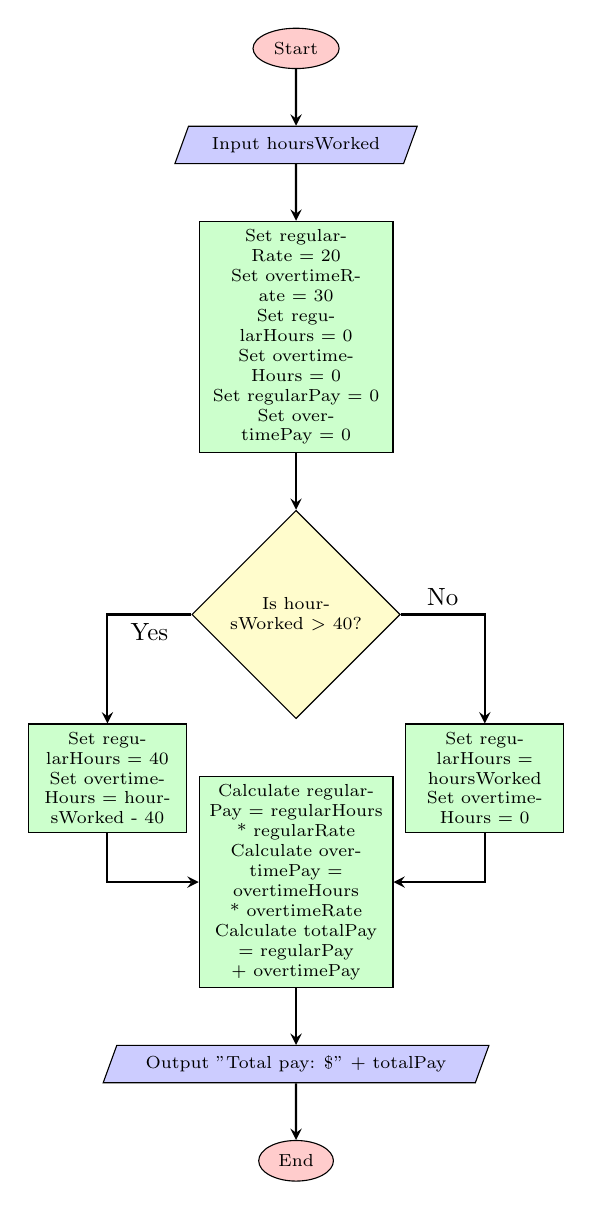
\begin{tikzpicture}[
        node distance=0.8cm and 0.8cm, % Reduced vertical and horizontal spacing
        auto,
        scale=0.9, % Scale the entire diagram to 90% of its original size
        transform shape % Ensure scaling applies to text and shapes
    ]
        % Nodes
        \node[startstop] (start) {Start};
        \node[inputoutput, below=of start] (input) {Input hoursWorked};
        \node[process, below=of input, text width=2.5cm] (init) {Set regularRate = 20\\Set overtimeRate = 30\\Set regularHours = 0\\Set overtimeHours = 0\\Set regularPay = 0\\Set overtimePay = 0};
        \node[decision, below=of init, text width=2cm] (decision) {Is hoursWorked \( > \) 40?};
        \node[process, below left=of decision, text width=2cm] (yes) {Set regularHours = 40\\Set overtimeHours = hoursWorked - 40};
        \node[process, below right=of decision, text width=2cm] (no) {Set regularHours = hoursWorked\\Set overtimeHours = 0};
        \node[process, below=of decision, text width=2.5cm] (calc) {Calculate regularPay = regularHours * regularRate\\Calculate overtimePay = overtimeHours * overtimeRate\\Calculate totalPay = regularPay + overtimePay};
        \node[inputoutput, below=of calc] (output) {Output "Total pay: \$" + totalPay};
        \node[startstop, below=of output] (end) {End};

        % Arrows
        \draw[arrow] (start) -- (input);
        \draw[arrow] (input) -- (init);
        \draw[arrow] (init) -- (decision);
        \draw[arrow] (decision) -| node[near start] {Yes} (yes);
        \draw[arrow] (decision) -| node[near start] {No} (no);
        \draw[arrow] (yes) |- (calc);
        \draw[arrow] (no) |- (calc);
        \draw[arrow] (calc) -- (output);
        \draw[arrow] (output) -- (end);
    \end{tikzpicture}
    \caption{Flowchart for Calculating Total Pay Based on Hours Worked}
    \label{fig:payroll_flowchart}
\end{figure}

\end{document}